\documentclass[11pt,a4paper]{article}

\usepackage[T1]{fontenc}
\usepackage[utf8]{inputenc}
\usepackage[margin=2.6cm]{geometry}
\usepackage{lmodern}
\usepackage{microtype}
\usepackage{graphicx}
\usepackage{booktabs}
\usepackage{amsmath}
\usepackage{caption}
\usepackage{subcaption}
\usepackage[numbers,sort&compress]{natbib}
\usepackage[hidelinks]{hyperref}
\usepackage{xcolor}
\usepackage{enumitem}

\captionsetup{font=small, labelfont=bf}
\setlist{itemsep=2pt, topsep=4pt}
\graphicspath{{figures/}}

% Default float parameters push large tables and figures onto pages of their
% own, leaving half-empty pages. These let floats share a page with body text.
\renewcommand{\topfraction}{0.90}
\renewcommand{\bottomfraction}{0.80}
\renewcommand{\textfraction}{0.08}
\renewcommand{\floatpagefraction}{0.80}
\setcounter{topnumber}{3}
\setcounter{bottomnumber}{2}
\setcounter{totalnumber}{4}

\newcommand{\prauc}{PR\nobreakdash-AUC}
\newcommand{\rocauc}{ROC\nobreakdash-AUC}

\title{\bfseries Predicting Overtakes in Formula One's 2026 Regulation Era:\\
\large A Discrete-Time Hazard Model under Extreme Data Scarcity}

\author{Amin Nami\\
\small MSc Bioinformatics, University of Bologna\\
\small \emph{Applied Machine Learning --- Advanced}}

\date{\today}

\begin{document}
\maketitle

\begin{abstract}
\noindent
Formula One's 2026 regulations replaced the Drag Reduction System with an
energy-based Overtake Mode, introduced active aerodynamics and moved to a
50/50 hybrid power unit. The mechanism of overtaking changed, so
models trained on earlier seasons do not transfer, yet only fourteen races of
in-era data exist. This paper addresses that cold-start problem. We reformulate
overtake prediction as a \emph{discrete-time hazard} over battle episodes with
censoring, which removes the overlapping-label defect of a fixed-horizon
classifier and recovers 706 observations a fixed-horizon formulation
discards. We adopt an expanding-origin backtest that yields ten out-of-sample
race results from fourteen rounds, and we transfer the pre-2026 era as a single
frozen scalar rather than as pooled rows. Our extraction reproduces published
season overtake totals to within 3.4\%. The final model reaches
\prauc{} 0.502 against a 6.58\% base rate (7.6$\times$
lift), \rocauc{} 0.911 and Brier 0.0438. Of eight design hypotheses
tested, six were overturned by measurement: a historical circuit passability
prior did not transfer ($\rho=+0.09$), monotone constraints had no effect,
hyperparameter tuning cost 1.2\%, and removing seven features
gained 5.1\%. Two held: an old-era model supplied as one feature
gained 4.2\% while improving nine of ten rounds, and circuit
\emph{physics} transferred ($\rho=+0.97$) where circuit \emph{outcome} did not.
A recurrent model over episode sequences did not beat gradient boosting. We
report all of it.
\end{abstract}

\section{Introduction}

Given two Formula One cars fighting on track, what is the probability that the
car behind completes a pass? The question is well posed and the data to answer
it is, in most seasons, plentiful. The 2026 season is not most seasons.

Three properties define the problem and drove every decision in this work.

\paragraph{The mechanism changed.} The 2026 regulations \citep{fia2026} removed
DRS and replaced it with an energy-based Overtake Mode, introduced active
aerodynamics with distinct straight and corner modes, and split the power unit
evenly between combustion and electrical power. Cars are 30\,kg
lighter with a 200\,mm shorter wheelbase. A model trained on
2022--2025 does not transfer unmodified, and a feature set built
around DRS zones describes a mechanism that no longer exists.

\paragraph{There is almost no in-era data.} At the time of writing, fourteen
races had been completed, yielding 470 passes across 6\,669 usable
observations. For comparison, the same pipeline applied to
2022--2025 produces roughly 49\,000 rows.

\paragraph{The era is ongoing.} A race is added every fortnight. The interesting
question is therefore not ``what is the best model on a fixed dataset'' but
``how should a model be built, evaluated and updated while the data keeps
arriving''. This motivates a walk-forward evaluation protocol and a retraining
loop rather than a single split.

\paragraph{Contributions.}
\begin{enumerate}[label=(\roman*)]
  \item A discrete-time hazard formulation of overtake prediction with proper
        censoring, which fixes three defects of the fixed-horizon framing
        (\S\ref{sec:formulation}).
  \item An evaluation protocol that extracts ten out-of-sample results from
        fourteen races and quantifies its own noise floor (\S\ref{sec:protocol}).
  \item A transfer mechanism that compresses four prior seasons into one frozen
        scalar, with measured gains and an ablation (\S\ref{sec:transfer}).
  \item A tested distinction between circuit properties that survive a
        regulation change and those that do not (\S\ref{sec:physics}).
  \item Six overturned hypotheses reported alongside two confirmed ones
        (\S\ref{sec:negative}).
\end{enumerate}

\section{Data}

\subsection{Source and reconnaissance}

All data comes from FastF1 \citep{fastf1}, which wraps Formula One's live
timing service. Only lap records, weather and race control messages are read;
car telemetry is never required, because the speed-trap measurements used here
are lap-level fields.

A reconnaissance pass established what 2026 actually exposes before any
modelling decision was taken. All fourteen completed rounds load
(16\,255 lap records, 22 drivers, 11 teams) and the lap schema is
identical to 2024. Critically, DRS is confirmed \emph{dead rather than
deprecated}: the telemetry channel still exists but all 35\,553 samples read
zero, against a live distribution in a 2024 reference race. No telemetry channel
exists for Overtake Mode, active aerodynamics or energy deployment.

\subsection{Defining and validating an overtake}

An overtake is detected as a \emph{pairwise order flip}: driver $A$ is behind
driver $B$ at the end of lap $L$ and ahead at the end of lap $L+1$. This is the
only definition available from timing data that references neither DRS, aero nor
energy, which is precisely why it survives the regulation change.

Raw flips overcount, because pit stops and retirements reorder the field without
an on-track pass. Pit-involved flips are excluded; lap one, safety-car periods
and inaccurate timing are retained, as they contain real passes.

Table~\ref{tab:validation} is the checkpoint on which everything downstream
depends.

\begin{table}[htbp]
\centering
\small
\caption{Extracted overtake counts against published figures, first four rounds
of 2026. The same detector applied to 2025 gives 77 against a published
84, so the method lands within roughly 10\% in both eras.}
\label{tab:validation}
\begin{tabular}{lrrr}
\toprule
Circuit & Published & Extracted & Difference \\
\midrule
Australian & 39 & 37 & $-2$ \\
Chinese    & 71 & 73 & $+2$ \\
Japanese   & 43 & 42 & $-1$ \\
Miami      & 50 & 58 & $+8$ \\
\midrule
\textbf{Total} & \textbf{203} & \textbf{210} & $+3.4\%$ \\
\bottomrule
\end{tabular}
\end{table}

\subsection{Reconstructing Overtake Mode}

Overtake Mode surfaces only as lap-stamped race control messages, and
reconstructing its state is less direct than it appears. Race control announces
an explicit disable only at the standing start; later neutralisations disable the
mode \emph{silently}, and the re-enable is announced inconsistently. Canada takes
virtual safety cars on laps 31, 46 and 53 and logs a re-enable
after each; Australia takes them on laps 12, 18 and 34 and logs
none. Replaying messages alone leaves Australia switched off for its final
46 laps.

The rule that survives all fourteen rounds uses track status as the primary
signal with messages as explicit overrides. Overtake Mode is available on
727 of 855 race laps (85.0\%).

\section{Exploratory analysis}

\subsection{Overtaking rose sharply and unevenly}

On the thirteen circuits raced in both seasons, passes rose 72\%
against 2025. The change is not a uniform multiplier: Monza more than tripled
($3.10\times$) while Barcelona fell to $0.56\times$. This single observation
drove the design decision in \S\ref{sec:physics}.

\subsection{Passes happen from very close range}

Figure~\ref{fig:gap} shows the gap distribution on the lap preceding a pass. The
median is 0.43\,s and the 99th percentile 2.36\,s.
This fixed the candidate threshold empirically: a 3.0\,s window
captures 98.9\% of passes, and widening to 4.0\,s buys a
further 0.3\% at the cost of 1\,161 additional rows.

\begin{figure}[htbp]
\centering
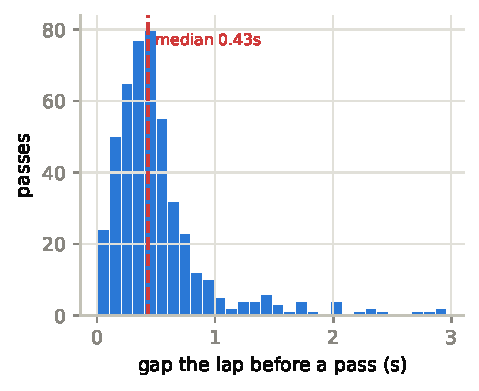
\includegraphics[width=0.52\textwidth]{gap_at_pass}
\caption{Gap on the lap before a completed pass. Overtaking is a close-range
phenomenon; the long tail is what makes the candidate threshold a real choice
rather than an obvious one.}
\label{fig:gap}
\end{figure}

\subsection{The target is rare and varies tenfold by circuit}

The overall base rate is 7.05\%, but per race it ranges from
1.1\% at Monaco (7 passes from 109 episodes) to
11.8\% at Monza (69 from 217). Any evaluation reporting
a single race's score measures the circuit as much as the model.

\section{Problem formulation}
\label{sec:formulation}

The natural formulation---``given this battle, will a pass occur within three
laps?''---has three defects.

\begin{enumerate}[label=(\alph*)]
  \item \textbf{Overlapping labels.} A pair battling on laps 12--14
        with a pass on 15 yields three rows, all labelled positive, with
        near-identical features. The model sees three examples and receives
        roughly one example of information.
  \item \textbf{Discarded information.} If the defender pits, the pass
        \emph{cannot} occur. Deleting such rows discards the genuine evidence
        that the pair fought for two laps without a pass.
  \item \textbf{A frozen horizon.} Three horizons require three label columns.
\end{enumerate}

We instead model the per-lap hazard, following standard discrete-time survival
practice \citep{singer2003applied,tutz2016modeling}:
\begin{equation}
h(t) = P\!\left(\text{pass on lap } t{+}1 \;\middle|\; \text{pair still battling at lap } t\right).
\label{eq:hazard}
\end{equation}
Any horizon follows by composition,
\begin{equation}
P(\text{pass within } k \text{ laps}) = 1 - \prod_{j=1}^{k}\bigl(1 - h_j\bigr),
\label{eq:horizon}
\end{equation}
so the horizon becomes a query parameter rather than a training decision.

Each row takes one of three outcomes. An \textbf{event} is a filtered on-track
pass between $L$ and $L+1$. \textbf{Survived} means no pass, and deliberately
includes the attacker dropping out of range, which is a genuine failure rather
than a missing observation; censoring it would bias the hazard upward by
discarding the clearest negatives available. \textbf{Censored} means the
opportunity was removed rather than declined---either car pitted, either car
retired, or the race ended. Censored rows carry no label but every earlier lap
of the episode is retained.

The resulting dataset comprises 860 episodes, 7\,491 rows of which
6\,669 are trainable, 470 events at a 7.05\% positive
rate, and a mean episode length of 8.71 laps. Censoring retains
706 pit-affected rows that a fixed-horizon formulation deletes outright.

\section{Evaluation protocol}
\label{sec:protocol}

The protocol was fixed \emph{before} any model was trained.

\paragraph{Expanding-origin backtest.} For each round $k$ from 5 to
14, we train on rounds $1\ldots k{-}1$ and predict round $k$
\citep{hyndman2021forecasting}. Every round becomes an out-of-sample test exactly
once, so fourteen rounds yield \emph{ten} test results rather than one. A
purpose-built test instruments the harness with a model that records which rounds
it trained on, verifying that round $k$ never appears in its own training set.

\paragraph{Frozen hyperparameters.} A 40-trial random search
\citep{bergstra2012random} ran on rounds 1--4 only, and the winner was
written to a committed file. A configuration chosen by inspecting round $k$ makes
round $k$ no longer out of sample.

\paragraph{Metrics.} \prauc{} is primary: the target is rare, and \rocauc{}
flatters classifiers under class imbalance \citep{davis2006relationship}. We also
report \rocauc{}, the Brier score \citep{brier1950verification} and expected
calibration error, because the model's output is displayed as a probability and
ranking quality alone does not establish that a stated 20\% means
twenty percent.

\paragraph{The noise floor.} Per-round \prauc{} has a standard deviation of
\textbf{0.228}. This figure governs how every subsequent result must be
read: a difference of 0.02 between two models is not a difference.

\section{Features and transfer}
\label{sec:transfer}

\subsection{Levels from 2026, shapes from the old era}

The overtake \emph{rate} is directly measurable from 2026 alone and belongs in
the intercept. What earlier seasons can supply is \emph{conditional} structure:
given a battle, what makes a pass likely. Pooling the two eras naively violates
this, because a single shared intercept across two base rates invites the model
to explain the difference using stale car performance.

Features are therefore tagged by transfer tier. \textbf{Tier 1}
(regulation-invariant) covers race state, positions, Overtake Mode state,
validated circuit character, and cross-race form computed from prior rounds only.
\textbf{Tier 2} (same meaning, shifted relationship) covers gap and gap dynamics,
pace and speed-trap \emph{deltas}, tyre and stint state. \textbf{Tier 3} is
excluded by construction and a unit test enforces its absence: all DRS features,
all \emph{absolute} car speeds and lap times, and team identity. Team identity is
dropped because 2026 fields eleven teams of which two have no history and the
remainder carry a performance level that is no longer true.

\subsection{The transfer mechanism}

The pre-2026 era enters as \emph{one frozen scalar per row}: the output of a
gradient-boosted model \citep{ke2017lightgbm} fitted once on 48\,932 legacy
rows across 2022--2025, reading the 43 features both eras share
and targeting a next-lap pass to match Equation~\ref{eq:hazard}. It never sees a
2026 row, so it cannot leak into any fold and requires no refitting. Four seasons
therefore reach the model as a single column, and disabling it makes the ablation
exact.

\subsection{Circuit physics transfers; circuit outcome does not}
\label{sec:physics}

An earlier design collapsed the circuit into a \emph{historical passability
prior}: a per-circuit overtake rate fitted on 2022--2025, on the
argument that levels shift but the ranking is geometry. Measured against the
thirteen comparable circuits, the Spearman rank correlation was
$\rho = +0.09$ ($p = 0.76$), and per-circuit ratios spanned
0.56--3.10. The hypothesis was rejected.

The mechanism explains the failure and supplies the replacement. Under DRS,
passability tracked zone length and slipstream; Overtake Mode is an \emph{energy}
aid, so what matters is full-throttle time. We therefore transfer circuit
\emph{physics} rather than circuit \emph{outcome}---a historical overtake rate
encodes what happened under a ruleset that no longer exists, whereas a speed trap
encodes the shape of a track the cars still drive. Crucially, the claim was
tested before being used (Table~\ref{tab:physics}).

\begin{table}[htbp]
\centering
\small
\caption{Rank correlation of per-circuit quantities between
2022--2025 and 2026, across the thirteen circuits raced in both eras.
Physics transfers; top speed---the one property the new power unit and active
aerodynamics actually changed---does not, and is excluded.}
\label{tab:physics}
\begin{tabular}{lrrl}
\toprule
Quantity & Spearman $\rho$ & $p$ & Decision \\
\midrule
Mid-sector speed trap & $+0.974$ & $<0.0001$ & retained \\
Straight dominance (top $/$ mid-sector) & $+0.967$ & $<0.0001$ & retained \\
Sector-1 speed trap & $+0.966$ & $<0.0001$ & retained \\
Race distance & $+0.999$ & $<0.0001$ & retained \\
\midrule
Top speed & $+0.461$ & $0.11$ & \textbf{excluded} \\
\midrule
\emph{Historical overtake rate} & $+0.09$ & $0.76$ & \textbf{rejected} \\
\bottomrule
\end{tabular}
\end{table}

\section{Models}

We compare a non-ML baseline, two linear models, two tree ensembles, a kernel
method, a feed-forward network and a recurrent model. Gradient boosting uses
monotone constraints encoding known physics. The comparison is reported in
full in \S\ref{sec:results}; the recurrent model is treated separately in
\S\ref{sec:sequence}.

\section{Results}
\label{sec:results}

\begin{table}[htbp]
\centering
\small
\caption{Pooled over ten backtest rounds (4\,680 rows, 308 events,
6.58\% base rate). Lift is \prauc{} relative to the base rate.
Against a per-round standard deviation of 0.228, the tree ensembles are
clearly ahead of everything else while the choice \emph{within} that family is
not resolvable.}
\label{tab:results}
\begin{tabular}{lrrrr}
\toprule
Model & \prauc{} & Lift & \rocauc{} & Brier \\
\midrule
Base rate                  & 0.057 & $0.9\times$ & 0.440 & 0.0617 \\
Gap alone                  & 0.323 & $4.9\times$ & 0.851 & 0.0514 \\
Logistic (5 features)      & 0.370 & $5.6\times$ & 0.874 & 0.0495 \\
SVM (RBF)                  & 0.418 & $6.3\times$ & 0.863 & 0.0531 \\
Multilayer perceptron      & 0.444 & $6.7\times$ & 0.878 & 0.0488 \\
GRU (pretrained)           & 0.453 & $6.9\times$ & 0.876 & 0.1018 \\
Logistic (all features)    & 0.462 & $7.0\times$ & 0.884 & 0.0460 \\
Random forest              & 0.493 & $7.5\times$ & 0.906 & 0.0457 \\
LightGBM                   & \textbf{0.515} & $\mathbf{7.8\times}$ & 0.909 & 0.0448 \\
\midrule
\textbf{LightGBM $+$ isotonic} (shipped) & 0.502 & $7.6\times$ & \textbf{0.911} & \textbf{0.0438} \\
\bottomrule
\end{tabular}
\end{table}

Table~\ref{tab:results} and Figure~\ref{fig:ladder} give the model comparison.
The shipped model applies isotonic calibration \citep{zadrozny2002isotonic},
surrendering a little \prauc{} for the best \rocauc{}, the best Brier score and a
threefold reduction in calibration error---the correct trade when the output is
displayed as a probability. Platt scaling \citep{platt1999probabilistic} was
tested and proved \emph{worse than no calibration} on this data
($\mathrm{ECE}=0.029$ against $0.014$ uncalibrated), and is not used.

\begin{figure}[htbp]
\centering
\begin{subfigure}[t]{0.49\textwidth}
  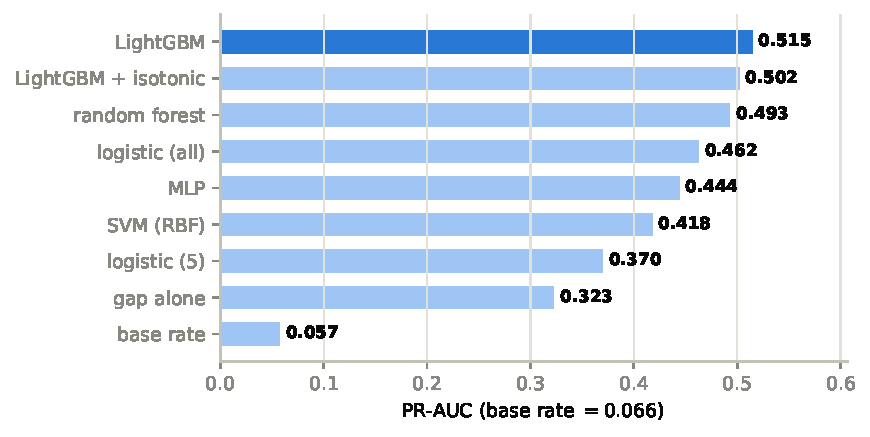
\includegraphics[width=\textwidth]{ladder}
  \caption{Model comparison.}\label{fig:ladder}
\end{subfigure}
\hfill
\begin{subfigure}[t]{0.49\textwidth}
  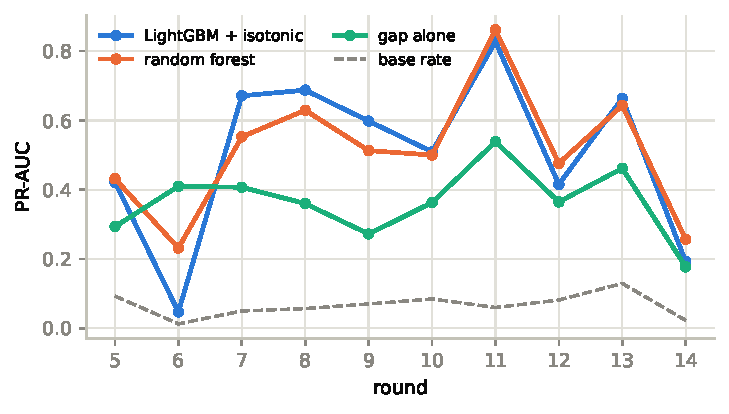
\includegraphics[width=\textwidth]{per_round}
  \caption{Per-round trajectory.}\label{fig:perround}
\end{subfigure}
\caption{Left: pooled \prauc{} by model. Right: \prauc{} for each backtest round.
The per-round variance ($\sigma = 0.228$) dwarfs the differences between the
leading models, which is why no single race can adjudicate between them.}
\end{figure}

\subsection{The transfer layer}

Supplying the pre-2026 era as one frozen scalar improves \prauc{} from
0.470 to 0.490 (+4.22\%) and improves \textbf{nine of
ten rounds}. Given the noise floor, the consistency carries more evidential
weight than the magnitude: nine of ten would arise by chance approximately
1\% of the time.

The result of interest is not the magnitude. The old-era model is \emph{weaker
alone than a single in-era feature}---\rocauc{} 0.768 against 0.862
for raw gap---yet it still improves the full model. It is therefore not
re-supplying gap; it carries structure the in-era model cannot recover from
fourteen races.

\subsection{Calibration and uncertainty}

Figure~\ref{fig:calib} shows the reliability curve of the shipped model. Isotonic
calibration reduces expected calibration error from 0.0142 to
0.0049.

Epistemic uncertainty is estimated by a bootstrap \citep{efron1979bootstrap}
resampled at \emph{race} level, since rows within a race are not independent.
Raw interval width is confounded by each test round's own hazard level, so width
is normalised by the predicted hazard. Interval width then narrows significantly
as the era accumulates data (Spearman $\rho = -0.649$, $p = 0.043$;
Figure~\ref{fig:intervals}). This is deliberately \emph{not} an accuracy claim:
see \S\ref{sec:overfit}.

\begin{figure}[htbp]
\centering
\begin{subfigure}[t]{0.42\textwidth}
  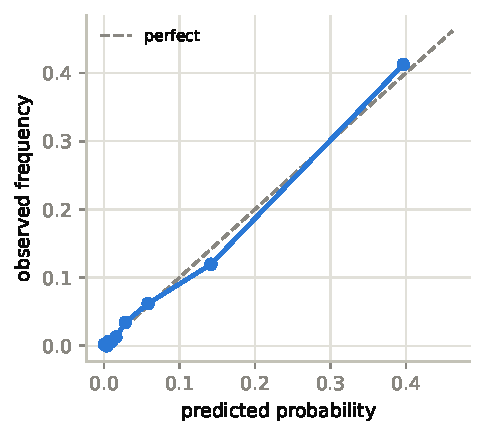
\includegraphics[width=\textwidth]{calibration}
  \caption{Reliability.}\label{fig:calib}
\end{subfigure}
\hfill
\begin{subfigure}[t]{0.42\textwidth}
  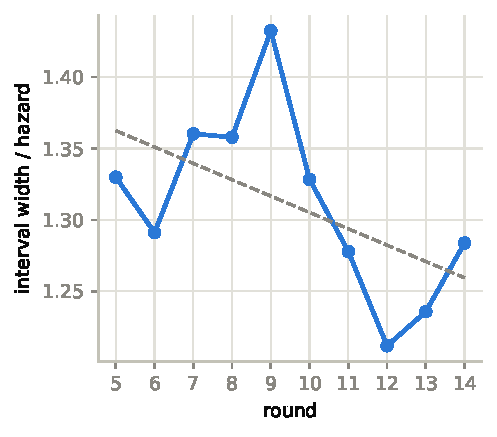
\includegraphics[width=\textwidth]{intervals}
  \caption{Interval width.}\label{fig:intervals}
\end{subfigure}
\caption{Left: predicted against observed frequency; points on the diagonal are
honest probabilities. Right: bootstrap interval width relative to the predicted
hazard, which narrows as rounds accumulate.}
\end{figure}

\section{Explainability}

Permutation importance \citep{altmann2010permutation} measured on held-out rounds
is cross-checked against TreeSHAP \citep{lundberg2017shap}. Both rank
\texttt{gap\_ahead} first and the \emph{transfer scalar second}, which is
independent confirmation of the ablation in \S\ref{sec:transfer}. All SHAP
directions are physically correct: a larger gap lowers the hazard, closing raises
it, a faster attacking team raises it.

\begin{figure}[htbp]
\centering
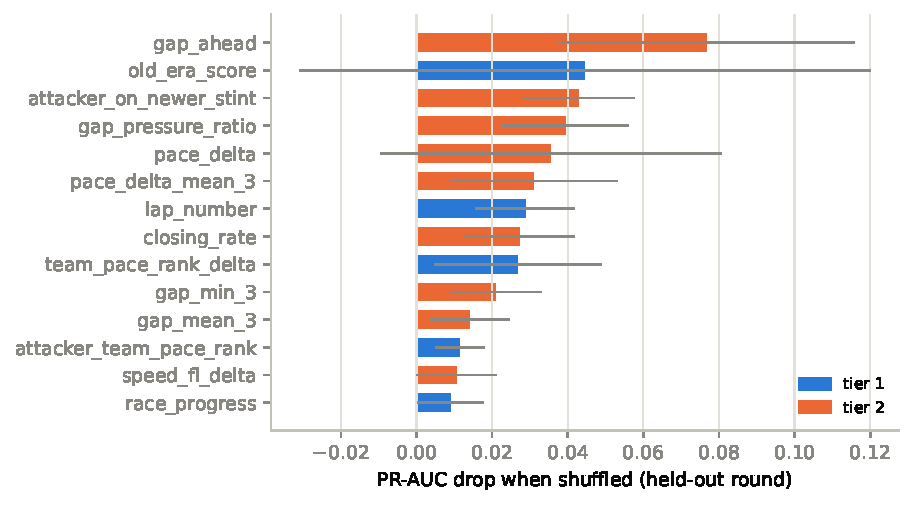
\includegraphics[width=0.72\textwidth]{permutation_importance}
\caption{Permutation importance on a held-out round, with standard deviation
across five shuffles. The transfer scalar \texttt{old\_era\_score} ranks second
of 57 features.}
\label{fig:importance}
\end{figure}

\paragraph{The feature set was over-engineered.} Of 57 features,
23 have zero or negative permutation importance. Removing the seven
features that are \emph{constant within a race}---weather, lap count, career
counters---raised \prauc{} from 0.489 to 0.515
(+5.1\%). The model had been using them as circuit fingerprints:
memorisation of which race it was looking at, which cannot generalise to an
unseen circuit. This was the largest single improvement in the project after the
transfer layer, and it came from \emph{removing} information. The validated
\texttt{circuit\_*} features are retained despite also being race-constant,
because they encode character shown to transfer rather than an incidental
identifier.

\section{Error analysis}

Sliced by circuit, the failures are concentrated and point one way
(Figure~\ref{fig:errors}). The model predicts 6.8\% at Monaco where
the truth is 2.0\%, and 6.9\% at Monza where the truth
is 12.7\%. \textbf{The two extremes of circuit passability are
precisely where the model breaks, in opposite directions.}

Adding validated circuit physics (\S\ref{sec:physics}) raised Monaco's \prauc{}
from 0.096 to 0.179 but barely moved the bias. Speed traps capture
how \emph{fast} a circuit is, not how \emph{passable}. Monaco is too narrow to
pass on at any speed, and track width, braking-zone count and corner-exit
geometry are not derivable from timing data at all. Closing this gap requires an
external geometry source and is the clearest single item of future work.

By gap band, calibration is otherwise excellent, with bias below 0.007 in
every band.

\begin{figure}[htbp]
\centering
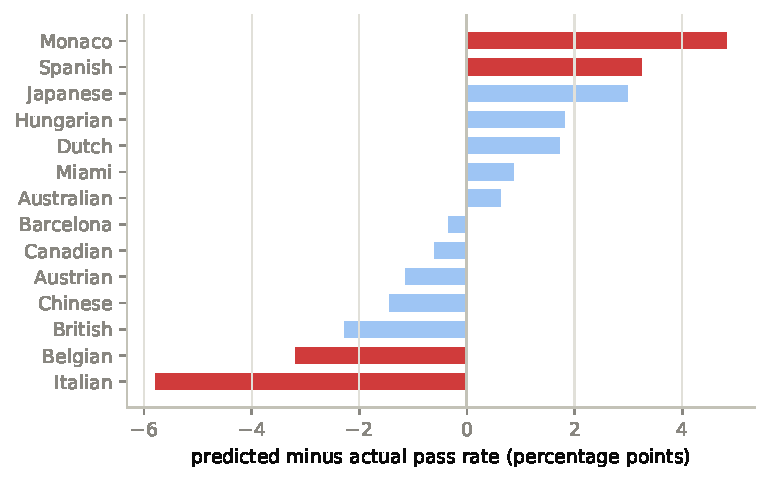
\includegraphics[width=0.72\textwidth]{error_by_circuit}
\caption{Predicted minus actual pass rate by circuit. Highlighted bars exceed
three percentage points. Monaco and Monza---the extremes of passability---fail in
opposite directions, which is the measurable cost of excluding circuit identity.}
\label{fig:errors}
\end{figure}

\section{Convergence and overfitting}
\label{sec:overfit}

Training on a growing prefix of rounds while always scoring the same held-out
race isolates training size from which race is predicted
(Figure~\ref{fig:learning}). Two conclusions follow.

First, the model \textbf{overfits heavily}: training \prauc{} sits near
0.96 at every training size against held-out values near 0.25, a
generalisation gap above 0.65 throughout. Second, and more importantly,
\textbf{additional data has not improved accuracy}. Held-out performance is flat
from two training rounds (0.279) to thirteen (0.252), consistent with
the per-round trajectory in Figure~\ref{fig:perround}, which shows no trend. The
extra data bought narrower \emph{uncertainty} (Figure~\ref{fig:intervals}) and
nothing else. The feature reduction reported above is the natural response;
stronger regularisation is the obvious next step.

\begin{figure}[htbp]
\centering
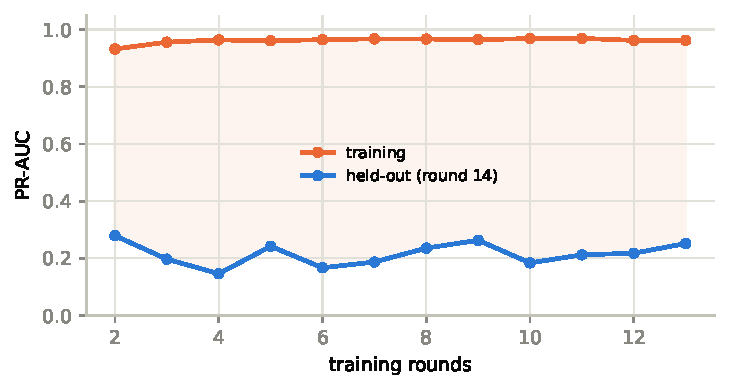
\includegraphics[width=0.72\textwidth]{learning_curve}
\caption{Learning curve. The shaded region is the generalisation gap. Training
performance is near-perfect at every size while held-out performance is flat,
indicating a model limited by the informativeness of the data rather than by its
quantity.}
\label{fig:learning}
\end{figure}

\section{The sequence model}
\label{sec:sequence}

Every other model treats a battle-lap as an independent row carrying
hand-computed history. A GRU \citep{cho2014gru} over the episode learns its own
summary instead, with identical features, target and protocol; the network is
unidirectional and the hazard head reads the hidden state at lap $t$, so no
future information leaks in.

It does not win (Table~\ref{tab:results}), which is the expected outcome on
heterogeneous tabular data at this sample size
\citep{grinsztajn2022tabular,shwartzziv2022tabular}. Two details matter more than
the headline. On \emph{ranking} the gap to LightGBM is within the noise floor;
where the GRU is clearly worse is \emph{calibration}, with a Brier score more than
twice as poor, which disqualifies it for a probability display regardless of
ranking. Second, pretraining the encoder on four prior seasons gained
0.3\%, against 4.22\% for the same era supplied as a
frozen scalar feature. \textbf{At this scale the old era transfers as a feature,
not as a representation}---the opposite of what the design predicted.

\section{Hypotheses overturned}
\label{sec:negative}

Eight design hypotheses were stated in advance and then tested. Six were
overturned (Table~\ref{tab:negative}), and several of the failures produced the
largest improvements in the final model.

\begin{table}[htbp]
\centering
\small
\caption{Design hypotheses against measured outcomes.}
\label{tab:negative}
\begin{tabular}{p{7.4cm}p{6.4cm}}
\toprule
Hypothesis & Outcome \\
\midrule
A historical circuit passability prior transfers & \textbf{Rejected.} $\rho=+0.09$, $p=0.76$ \\
Monotone constraints help at small $n$ & \textbf{No effect.} $0.4662$ vs $0.4641$ \\
Cross-race form is the largest remaining gap & \textbf{Marginal.} $+0.8\%$; in-race pace already subsumes it \\
Hyperparameter tuning improves the model & \textbf{Rejected.} $-1.2\%$; the search selected noise \\
Pretraining is where a sequence model wins & \textbf{Rejected.} $+0.3\%$ \\
More features are better & \textbf{Rejected.} Removing seven gained $+5.1\%$ \\
\midrule
An old-era model as one feature is the best transfer & \textbf{Confirmed.} $+4.22\%$, better in 9/10 rounds \\
Circuit \emph{physics} transfers where \emph{outcome} did not & \textbf{Confirmed.} $\rho=+0.97$ \\
\bottomrule
\end{tabular}
\end{table}

The frozen tuned parameters remain the default despite being 1.2\%
worse than a hand-chosen prior, because adopting the prior \emph{after} observing
it win on the test rounds is exactly the post-hoc selection the protocol exists
to prevent.

\section{Reproducibility and operations}

The project is an installable Python package with 88 tests. A retraining
loop is implemented and runnable but deliberately dormant: the incumbent scores
each new race \emph{before} anything is retrained, so evaluation and drift
detection are a single computation; the promotion gate compares
\emph{configurations} walked forward over five rounds rather than fitted objects
over rounds the challenger has already seen; and the drift monitor reports only
what its sample size supports, holding race-level features silent until a second
season exists.

\section{Limitations}

\begin{enumerate}[label=\arabic*.]
  \item \textbf{Fourteen races.} 470 events is a small sample and every
        conclusion should be read against $\sigma = 0.228$.
  \item \textbf{Circuit passability remains unrepresented.} Physics was
        validated and helped, but width, braking zones and corner-exit geometry
        are not obtainable from timing data.
  \item \textbf{Overtake Mode is observable but not identifiable.} Its
        availability correlates with track neutralisation at $-0.954$: the aid is
        withdrawn essentially only when passing is forbidden anyway, leaving
        49 of 6\,669 rows as green-track-with-mode-off. The feature is
        retained but credited with nothing.
  \item \textbf{Per-car energy deployment is invisible.} Whether a driver had
        energy banked and chose to spend it is not exposed in any channel.
  \item \textbf{No cross-era validation of the transfer claim.} The
        4.22\% is measured within 2026 only.
\end{enumerate}

\section{Conclusion}

Overtake prediction in a new regulation era is a cold-start problem, and this
work treats it as one. Reformulating the target as a discrete-time hazard with
censoring recovers information a fixed-horizon classifier discards; an
expanding-origin protocol extracts ten out-of-sample results from fourteen races
and quantifies its own noise floor; and compressing four prior seasons into a
single frozen scalar transfers useful structure while leaving the new era's base
rate untouched.

The most useful outcome may be the negative results. Six of eight stated
hypotheses were overturned, and the two largest improvements in the final model
came from \emph{rejecting} a designed component and from \emph{removing}
features. The model is limited by the informativeness of fourteen races rather
than by their quantity, and its failures are concentrated at precisely the two
circuits whose character it was forbidden to memorise.

\section*{Declaration of LLM use}

\emph{[To be reviewed and signed by the author.]} A large language model
assistant was used for implementation, debugging and drafting, in accordance with
the course's fair-use guidance. It was used to write and refactor code, to draft
this report from the project's own measured results, and to propose analyses.
Every methodological claim herein is supported by a measurement recorded in the
project's version history rather than by assertion, and the project's rejected
hypotheses are reported alongside its confirmed ones. The author is responsible
for, and able to justify, every choice, parameter, result and interpretation in
this report.

\bibliographystyle{plainnat}
\bibliography{references}

\end{document}
